%\documentclass[draft,grl]{AGUTeX}
\documentclass[twocolumn,grl]{AGUTeX}
\usepackage{mathptmx}
% \usepackage{lineno}
% \linenumbers*[1]

%  To add line numbers to lines with equations:
%  \begin{linenomath*}
%  \begin{equation}
%  \end{equation}
%  \end{linenomath*}

%  Uncomment the following command to include .eps files
%  (comment out this line for draft format):
%\usepackage[dvips]{graphicx}
\usepackage[pdftex]{graphicx}
%\setkeys{Gin}{draft=false}

\authorrunninghead{STYRON AND HETLAND}
\titlerunninghead{LANF EARTHQUAKE LIKELIHOOD}

\authoraddr{Corresponding author: Richard H. Styron,
Department of Earth and Environmental Sciences, University of
Michigan, 2534 CC Little Bldg., 1100 N. University Ave., 
Ann Arbor, MI 48104, USA (richard.h.styron@gmail.com)}

\begin{document}
\title{Likelihood of observing an earthquake on a low-angle normal fault}

\authors{Richard H. Styron \altaffilmark{1}
and Eric A. Hetland \altaffilmark{1}}

\altaffiltext{1}{Department of Earth and Environmental Sciences, University of
Michigan, Ann Arbor, Michigan, USA.}

\begin{abstract}
rothko
The recognition of low-angle normal faults, or LANFs, with fault dips less than 30$^\circ$ in the geologic record and their hypoth- esized role in accommodating large-magnitude continental exten- sion [Wernicke, 2009] has been one of the most important develop- ments in tectonics over the past several decades. However, despite widespread field observations of inactive LANFs[2] and their cen- tral role in modern extensional tectonic theory[3], they remain enig- matic and contentious structures. This is for two reasons: because brittle faulting on LANFs is in apparent conflict with standard rock mechanical theory as typically applied to the upper crust [4,5], and because observations of active faulting on LANFs is sparse and at times ambiguous[6,7]. A considerable amount of research has been performed to address the former concern, reconciling LANF slip with rock mechanics.
\end{abstract}

\begin{article}

\section{Introduction}
Low-angle normal faults (LANFs), with dips less than 30$^\circ$, are well described in the geologic record. They are hypothesized to have an important role in accommodating large-magnitude continental extension \citep{howard1987crustal} and crustal thinning \citep{lister1986detachment}, and their recognition has been one of the most important developments in tectonics over the past several decades \citep{wernicke2009detachment}. However, despite widespread field observations of inactive LANFs and their central role in modern extensional tectonic theory, they remain enigmatic and contentious structures. This is for two reasons: because brittle faulting on LANFs is in apparent conflict with standard Andersonian rock mechanical theory as typically applied to the upper crust \citep{axen2004lanfmech}, and because observations of active faulting on LANFs is sparse and at times ambiguous \citep{wernicke1995seis,}. A considerable amount of research has been performed to address the former concern, reconciling LANF slip with rock mechanics. The latter issue, the paucity of observations, has inhibited hypothesis testing of LANF fault theory, and has also contributed to a mode of thought where the absence of evidence for LANF activity is taken as evidence of its absence \citep{jackson1987, collettinisibson2001}. Alternately, the lack of observed seismic slip on a continental LANF may be explained by the rarity of seismicity and the small number of potential active structures.

In this work, we choose to directly address the question of whether the lack of observed seismicity may be interpreted as an indication that LANFs may not slip seismically, or is an effect of a small sample size of LANFs that show typical seismic behavior.  We do this by calculating the likelihood of observing a moderate to large earthquake on a LANF over different time windows, assuming that all continental LANFs described in the literature are seismically active at low angles and display typical seismic behavior.

\subsection{Mechanical Aspects of LANF Slip}



\section{Potentially Active LANFs}

Over the past decade or so, many field studies have found evidence for LANF activity in orogens throughout the world. These studies typically find arrays of Quaternary normal fault scarps on the fault traces and/or in the hanging walls of mapped or inferred low-angle detachment faults \citep [e.g.,][]{axen1999baja}. Some studies also have bedrock thermochronology data from the exhumed footwalls of the detachments that is suggestive of ongoing rapid exhumation \citep [e.g.,][]{sundell2013lunggar}, although this data does not preclude a recent cessation of faulting. In some cases, additional evidence for LANF activity comes from geophysical data such as GPS geodesy \citep [e.g.,][]{hreinsdottir2009altotib} and seismic waves \citep [e.g.,][]{doser1987ancash}.

We have compiled all potentially active LANFs with known subareal fault traces from a thorough review of the literature; there are nineteen total (Figure~\ref{fig:lanf_map}).  About half are in Tibet, consistent with hypotheses that LANFs and metamorphic core complexes form in areas of hot, thick crust \citep [e.g.,][]{buck1991mcc}.  The rest are distributed through other areas of active continental extension: the North American Basin and Range, the Malay Archipelago, Turkey, Italy, and Peru. Several of the most-commonly cited candidates for seismically active LANFs were not included because they do not have a clearly-defined, mappable fault trace, which is necessary for our calculations.  These include the submarine core complexes in the Woodlark Basin \citep{abers2001}, the fault responsible for the 1995 Aigion, Greece earthquake \citep{bernard1997} and other potential LANFs underneath the Gulf of Corinth, and the fault responsible for the 1952 Ancash, Peru earthquake \citep{doser1987ancash}.


\begin{figure*}
\noindent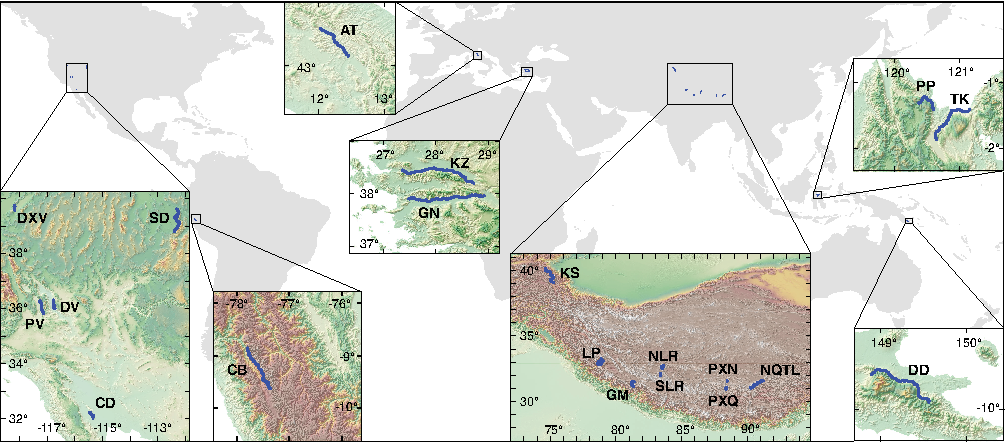
\includegraphics[width=40pc]{./figures/active_lanfs_map_insets.pdf}
\caption{Map of known, potentially active continental LANFs (blue lines), with insets showing the physiographic context of the faults.  DXV=Dixie Valley fault.  PV=Panamint Valley fault.  DV=Death Valley fault.  LS=Laguna Salada fault.  CB=Cordillera Blanca detachment.  AT=Alto-Tiberina fault.  KZ=Kuzey detachment.  GN=Guney detachment.  KS=Kongur Shan fault.  LP=Leo Pargil detachment.  GM=Gurla Mandhata detachment. NLR=North Lunggar detachment.  SLR=South Lunggar detachment.  PXN=Pum Qu--Xainza north fault.  PXQ=Pum Qu--Xainza Qingdu fault.  NQTL=Nyainqentanglha detachment.  PP=Papangeo detachment.  TK=Tokorondo detachment.  DD=Dayman Dome.}
\label{fig:lanf_map}
\end{figure*}

We have then mapped the approximate fault traces into a GIS file (available at https://github.com/cossatot/LANF\_gis), with metadata such as slip rate and source. We then have estimated the probability of observing an earthquake above a given magnitude for each fault individually over some time window, and then calculated the probability of observing a significant earthquake on any of the faults over that same time window.

\section{Likelihood of observing a LANF event}
\subsection{Rupture Likelihood on Individual LANFs}
To estimate the likelihood of observing a significant earthquake on an individual LANF over some contiguous time window of length $t$ (in years), we perform a Monte Carlo simulation in which we create 2000 synthetic time series of earthquakes, with unique values for fault geometry and slip rate for each time series. Then, for each time series we calculate the fraction of unique time windows of length $t$ in which an earthquake as large or larger than a given magnitude occurs.  We take this value as the probability of observing an earthquake greater than or equal to moment magnitude \emph{M} in time $t$, which we will refer to in the general sense as $P(M,t)$.

The geometry for each fault is estimated based on the length of the fault trace, the dip of the fault, and the estimated seismogenic thickness or fault locking depth in the area.  The fault is treated as planar for simplicity of calculations, even though the exposed footwalls of many detachment faults are highly corrugated.  We determine the fault length by measuring the approximate length of the mapped fault trace perpendicular to the assumed extension direction; for faults that change dip significantly along strike (e.g., the Dixie Valley fault), we only consider the low-angle segments of the fault.  Values for the dip are taken from the literature in most cases, and measured from SRTM data otherwise; in all cases, a range of values is considered.  The seismogenic thickness or fault locking depth is assumed to be 10 km in the absence of other evidence (such as a geodetic study, \citep [e.g.,][]{hreinsdottir2009altotib}).

Slip rates are similarly gathered from the literature if possible, or given broad ranges if not (e.g., 1--10 mm yr$^{-1}$).  In the Monte Carlo simulation, samples for slip rate and dip are drawn from uniform distributions defined by the maximum and minimum values.  Based on field observations, some faults have dip ranges that go above 30$^\circ$; this study only considers slip on faults shallower than this, so for these faults, dip values are sampled from the minimum to 30$^\circ$ and the resulting probabilities are then multiplied by the fraction of the dip range that is under 30$^\circ$.

Each earthquake sequence is generated by randomly sampling 50,000 events from a tapered Gutenberg-Richter distribution with corner magnitude $M_c = 7.64$ and $\beta = 0.65$ (from values estimated by \citet{birdkagan2004f_m} for continental rifts) using an inverse transform sampling algorithm.  The samples are taken from a moment magnitude interval $M = [5.0, \, M_{max}]$, where $M_{max}$ is calculated as the magnitude M resulting from fault slip $D$ = 15 m over a fault of length $L$ cutting through a seismogenic thickness $z$ at dip $\delta$, given the relations 

\begin{equation}
 M_o = \mu L z D \,/ \, \sin \delta 
 \end{equation}

and

\begin{equation}
M = 2/3 \; \log_{10} (M_o) - C 
\end{equation}
where $C = 6 $ and shear modulus $\mu = 30$ GPa.  Sensitivity tests (see Supplementary Materials) show that the results are only slightly affected by the frequency-magnitude distribution: differences between results using this distribution and a `characteristic' distribution with an enhanced probability of earthquakes around $M$ 6 are well below the variability created by uncertainty in fault dip and slip rate.  

Then, a time series of strain accumulation and release for each earthquake sequence is created, with one value per year.  This is constructed by separating each earthquake from the previous one with a set of zeros (representing no significant earthquakes for those years) where the number of zero years before an event corresponds to the length of an interseismic interval necessary to accumulate all the slip released in that event, given the fault dimensions and slip rate for that time series. Then, the likelihood of observing a significant earthquake is calculated as described above.

As an example, the results for the Kongur Shan fault are shown in Figure~\ref{fig:kongur_all_probs} a.  The results show that it is unlikely that any earthquake above \emph{M} 5.0 will be observed over time scales up to a century. 

\begin{figure}[ht!]
\noindent\includegraphics[width=20pc]{./figures/kongur_all_probs.pdf}
\caption{\textbf{a:} Probabilities of observing an earthquake greater than or equal to a given moment magnitude \emph{M} over a given observation window on the Kongur Shan fault (Tibet). \textbf{b:} Probabilities of observing an earthquake greater than or equal to a given moment magnitude \emph{M} over a given observation window on all studied LANFs. }
\label{fig:kongur_all_probs}
\end{figure}


\subsection{Probability on All LANFs}
To calculate the probability of observing an earthquake over the time window on any of the LANFs studied, we first assume that seismicity on each fault is independent and uncorrelated from seismicity on all other faults. This assumption is likely true for most faults, but may not be true for some proximal faults (such as the North and South Lunggar detachments, or the Papangeo and Tokorondo detachments), though it is hard to determine how these faults may interact.  We determine the probability for each time window and minimum magnitude with the equation
\begin{equation}
p_{AT \, or \, LP\, \ldots \, or \, DV} = 1 - (q_{AT} \cdot q_{LP} \cdot \ldots \, \cdot q_{DV})
\end{equation}
where $p_{AT}$ is the probability of observing an earthquake on a single LANF (the Alto-Tiberina fault), and $q_{AT} = 1 - p_{AT}$.

The results of this calculation are shown in Figure~\ref{fig:kongur_all_probs} b.  Unlike the results from a single fault, the results from all faults show that it is likely that a significant earthquake on a LANF would be observed over an observation period of even a handful of years.  If we take \emph{M} 6.0 as the lowest magnitude for which modern, global earthquake catalogs are complete [e.g., ref], and 40 years as the length of those catalogs, then the probability of seeing a significant LANF event is about 0.65.

Here we need a better introduction to the next section.

\subsection{Possible Effect of Inactive Faults}
Of the faults considered here, several have received little to no field study, and others have generated conflict in the literature over whether they are active.  It is possible that these faults spuriously affect the results, raising $P(M,t)$.  To test this, we re-run the final calculations, disregarding the Tokorondo and Papangeo detachments (as they have received no modern field study and do not have clear Quaternary fault scarps in Google Earth imagery), and the Kuzey and Guney detachments, as evidence exists that they are inactive [e.g., refs, G. Axen, personal communication].  Because the smaller faults with lower slip rates do not significantly impact the results (see Supplementary Materials), we do not leave out other poorly-studied or contested faults.
	
The results from the calculations without these faults are shown in Figure~\ref{fig:all_probs_no_maybes} a. The probabilities for the reference  


\begin{figure}%[t!]
\noindent\includegraphics[width=20pc]{./figures/all_M_no_maybes.pdf}
\caption{\textbf{a:} Probabilities of observing an earthquake greater than or equal to a given moment magnitude \emph{M} over a given observation window on the all faults except those in Turkey and Sulawesi. \textbf{b:} Component of total probabilities contributed by the Turkey and Sulawesi faults.}
\label{fig:all_probs_no_maybes}
\end{figure}


\section{Discussion and conclusions}

This compilation of nineteen potentially active LANFs shows that they are uncommon structures, but they may be found in areas of active extension, particularly in hot, thick crust such as Tibet and the Andes. 
Though the fault traces of many LANFs considered here are obscured by vegetation or agriculture, others display large fault scarps in Quaternary sediments, particularly those in the dry climates of Tibet \citep[e.g.,][]{styron2013slr, kapp2005nqtl} and the western US \citep[e.g.,][]{axen1999baja, heyman2003dv}, which are not known to be associated with creeping faults.









% put bib here

\end{article}

%\begin{figure}
%\noindent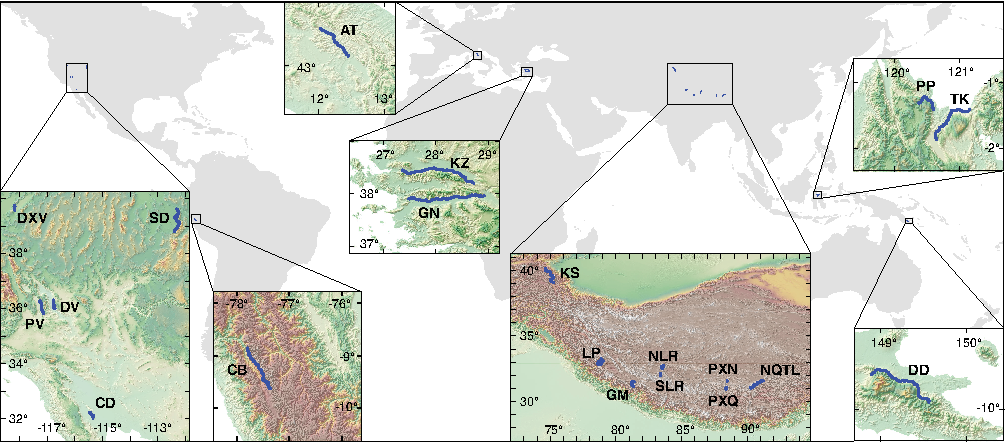
\includegraphics[width=40pc]{./figures/active_lanfs_map_insets.pdf}
%\caption{Map of known, potentially active continental LANFs (blue lines), with insets showing the physiographic context of the faults.  DXV=Dixie Valley fault.  PV=Panamint Valley fault.  DV=Death Valley fault.  LS=Laguna Salada fault.  CB=Cordillera Blanca detachment.  AT=Alto-Tiberina fault.  KZ=Kuzey detachment.  GN=Guney detachment.  KS=Kongur Shan fault.  LP=Leo Pargil detachment.  GM=Gurla Mandhata detachment. NLR=North Lunggar detachment.  SLR=South Lunggar detachment.  PXN=Pum Qu--Xainza north fault.  PXQ=Pum Qu--Xainza Qingdu fault.  NQTL=Nyainqentanglha detachment.  PP=Papangeo detachment.  TK=Tokorondo detachment.  DD=Dayman Dome.}
%\label{fig:lanf_map}
%\end{figure}

%\begin{figure}
%\noindent\includegraphics[width=20pc]{./figures/kongur_all_probs.pdf}
%\caption{\textbf{a:} Probabilities of observing an earthquake greater than or equal to a given moment magnitude \emph{M} over a given observation window on the Kongur Shan fault (Tibet). \textbf{b:} Probabilities of observing an earthquake greater than or equal to a given moment magnitude \emph{M} over a given observation window on all studied LANFs. }
%\label{fig:kongur_all_probs}
%\end{figure}


%\begin{figure}
%\noindent\includegraphics[width=20pc]{./figures/kongur_all_probs.pdf}
%\caption{\textbf{a:} Probabilities of observing an earthquake greater than or equal to a given moment magnitude \emph{M} over a given observation window on the Kongur Shan fault (Tibet). \textbf{b:} Probabilities of observing an earthquake greater than or equal to a given moment magnitude \emph{M} over a given observation window on all studied LANFs. }
%\label{fig:kongur_all_probs}
%\end{figure}

%\bibliographystyle{agufull08}
%\bibliography{styron_hetland_lanf.bib}

\end{document}


